\documentclass[usenames,dvipsnames]{beamer}
\usetheme{Boadilla}
\usecolortheme{whale}

\usepackage[T1,T2A]{fontenc}
\usepackage[utf8]{inputenc}
\usepackage[english,russian]{babel}	% Localization
\usepackage{appendixnumberbeamer}
%\useinnertheme[shadow=true]{rounded}

\usepackage{amsmath,euscript,mathrsfs}
\usepackage{amssymb,amsfonts,latexsym,mathtools}
\usefonttheme[onlymath]{serif}
\usepackage{graphicx} 
\usepackage{wrapfig}
\usepackage{xcolor}
\usepackage{booktabs}

\usepackage{caption,tabularx,subcaption}
\usepackage{animate}

% Absolute value declaration
\DeclarePairedDelimiter{\abs}{\lvert}{\rvert}
\DeclarePairedDelimiter{\norm}{\|}{\|}
\DeclareMathOperator{\erf}{erf}
\DeclareMathOperator{\trace}{tr}
\DeclareMathOperator{\sech}{sech}

% Page breaking in multi-line formulae
\allowdisplaybreaks[1]

% Delimiters
\newcommand{\lb}{\left (}
\newcommand{\rb}{\right )}
\newcommand{\lset}{\left \{}
\newcommand{\rset}{\right \}}
\newcommand{\lsq}{\left [}
\newcommand{\rsq}{\right ]}

% Tensors
\newcommand{\vect}[1]{\underline{#1}}
\newcommand{\tens}[1]{\underline{\underline{#1}}}

% Additional commands
\newcommand{\divg}{\text{div}}

% Big 'O' notation
\renewcommand{\O}[1]{O \lb #1 \rb}

% Equation specific commands
\newcommand{\eqtext}[1]{\quad \text{#1} \quad}
\newcommand{\RA}{\quad \Rightarrow \quad}

% Derivatives (normal and partial)
\newcommand{\dd}[1]{\; \mathrm{d} #1}
\newcommand{\diff}[2]{\frac{\mathrm{d} #1}{\mathrm{d} #2}}
\newcommand{\diffn}[3]{\dfrac{\mathrm{d}^{#1} #2}{\mathrm{d} #3^{#1}}}
\newcommand{\pdd}[1]{\; \partial #1}
\newcommand{\pdiff}[2]{\frac{\partial #1}{\partial #2}}
\newcommand{\pdiffn}[3]{\dfrac{\partial^{#1} #2}{\partial #3^{#1}}}

\setlength{\abovedisplayskip}{0pt}
\setlength{\belowdisplayskip}{1pt}

\setbeamercolor{block body}{bg=Blue}%bg=background, fg= foreground

\defbeamertemplate*{title page}{customized}[1][]
{
	\centering
	{\footnotesize
	Санкт-Петербургский политехнический университет Петра Великого\\
	Институт прикладной математики и механики\\
	}
	\vspace{12mm}
	Выпускная квалификационная работа магистра\\
	\vspace{3mm}
	\usebeamerfont{title}\inserttitle\par
	\bigskip
}


\title[Волны в нелинейно упругих стержнях]{Продольные волны деформации в нелинейно упругих волноводах}
\author[Ф.\,Е. Гарбузов]{Ф.\,Е. Гарбузов}

\begin{document}

%\frame[plain]{\titlepage}

%\maketitle

\begin{frame}[plain]
\centering
{\footnotesize
Санкт-Петербургский политехнический университет Петра Великого\\
Институт прикладной математики и механики
}

\vspace{12mm}
Выпускная квалификационная работа магистра
\vspace{3mm}

\begin{block}{}
	\centering
	\Large\color{white}
	Продольные волны деформации в нелинейно упругих волноводах
\end{block}
\vspace{12mm}

{ \footnotesize 
\begin{tabularx}{.9\linewidth}{Xr}
	Выполнил студент гр. 23641/1 \vspace{2mm}& Ф.\,E.~Гарбузов\\
	Руководитель, д.т.н., проф. (СПб\,ПУ)\vspace{2mm} & Б.\,С.~Григорьев\\
	Научный консультант, к.ф.-м.н. (ФТИ им. Иоффе) & Я.\,М.~Бельтюков\\
\end{tabularx} 
}
\end{frame}


\begin{frame}{Актуальность}
	%\animategraphics[loop,controls,width=.5\linewidth]{}{Anim/sol}{1}{30}
	В нелинейно упругих волноводах могут возникать солитоны деформации.\\
	\vspace{2mm}
	Солитоны:
	\begin{itemize}
		\item могут распространяться на большие расстояния;
		\item способны фокусироваться при сужении волновода $\Rightarrow$ приводить к сильным деформациям;
		\item сохраняют память о прохождении через область с дефектом\\ $\Rightarrow$ могут быть применены в дефектоскопии.
	\end{itemize}
	\vspace{2mm}
	Стержень при прохождении солитона сжатия:
	\begin{figure}
		\vspace{-2mm}
		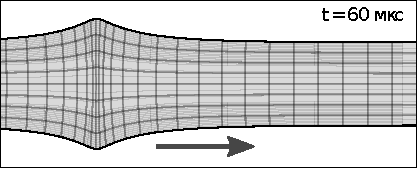
\includegraphics[width=0.46\linewidth]{Figures/DeformedRod1}
		\hspace{5mm}
		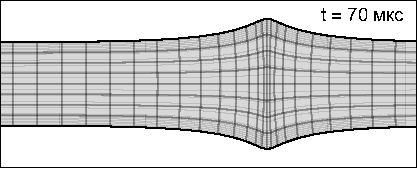
\includegraphics[width=0.46\linewidth]{Figures/DeformedRod2}
	\end{figure}
\end{frame}

 
\begin{frame}{Задачи}
\begin{enumerate}
	\item Вывести одномерное уравнение для продольных волн в нелинейно упругом стержне, учитывающее заданные на поверхности напряжения.
	\item Проанализировать свойства выведенного уравнения и найти его солитонные решения. 
	\item Провести серию численных экспериментов по генерации солитонов деформации. Сравнить решения выведенного одномерного уравнения с решениями полных трёхмерных уравнений движения.
\end{enumerate}
\end{frame}


\begin{frame}{Полные трёхмерные уравнения}
\begin{wrapfigure}[6]{r}{125pt}
	\vspace{-2mm}
	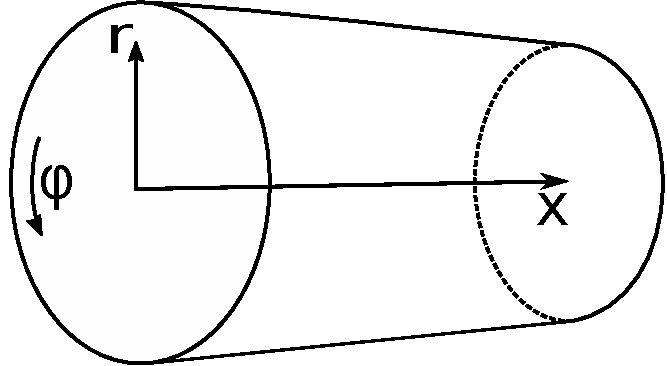
\includegraphics[width=\linewidth]{Figures/1_RodSchematic}
\end{wrapfigure}
Трёхмерный вектор перемещения $\color{black}\vect{U}$.\\
\vspace{1mm}
Нелинейный тензор деформации:
\begin{equation*}
\tens{E} = \frac12 \lb(\nabla\vect{U})^T + \nabla\vect{U} + {\color{blue}(\nabla\vect{U})^T\cdot\nabla\vect{U}}\rb
\end{equation*}
Определяющее соотношение Мурнагана:
\small
\begin{align*}
&W = \frac{\lambda + 2\mu}{2}I_1(\tens{E})^2 - 2\mu I_2(\tens{E}) +\color{blue} \frac{l+2m}{3}I_1(\tens{E})^3 - 2m I_1(\tens{E}) I_2(\tens{E}) + n I_3(\tens{E})
\end{align*}
$\lambda,\ \mu$ --- модули упругости Ламе (линейные),\\
$\color{blue}l,\ m,\ n$ --- модули упругости Мурнагана (нелинейные).\\
\vspace{1mm}
\normalsize
Полные трёхмерные уравнения движения:
\begin{equation}\nonumber
%\color{blue}
\rho\ddot{\vect{U}} = \divg\tens{P}, \qquad \tens{P} = (\tens{I} + \nabla\vect{U}) \cdot \pdiff{W}{\tens{E}}
\end{equation}
На границе стержня задано напряжение $\vect{P}_b$:
\begin{equation}\nonumber
\tens{P}\cdot \vect{n} = \vect{P}_b
\end{equation}
\end{frame}


\begin{frame}{Упрощение полных уравнений}
\begin{itemize}%[noitemsep,topsep=1pt]
	\hspace{-3mm}
	\begin{minipage}{.53\textwidth}
	\item Стержень бесконечен вдоль оси $x$
	\item Нет кручения, от угловой координаты $\varphi$ ничего не зависит
	\item Масштаб пространственных переменных: $\color{black}x,\ r \sim L$
	\item Тонкий стержень: $\color{black}R/L = \delta \ll 1$
	\item Масштабы перемещений: $\color{black}U,\ V \sim \varepsilon L$
	\item Малые деформации: $\color{black}\pdiff{U}{x},\ \pdiff{V}{r} \sim \varepsilon \ll 1$
	\end{minipage}
	\hspace{3mm}
	\begin{minipage}{.36\textwidth}
		%\vspace{-2mm}
		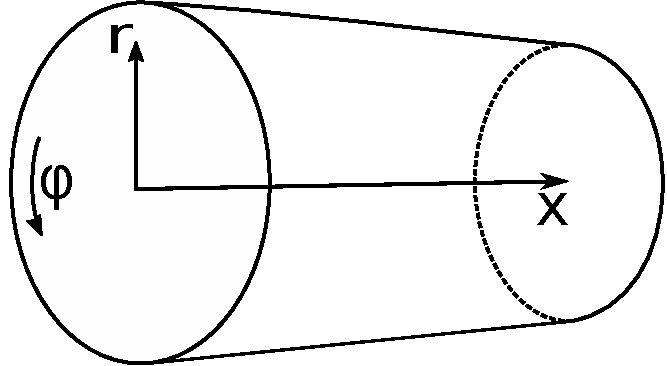
\includegraphics[width=\linewidth]{Figures/1_RodSchematic}\\
		\footnotesize
		Радиус стержня --- $R$.\\
		Перемещения:\\
		$U$ --- осевое (продольное), \\
		$V$ --- радиальное (поперечное).
	\end{minipage}
\end{itemize}
\setlength{\belowdisplayskip}{1pt} \setlength{\belowdisplayshortskip}{0pt}
\setlength{\abovedisplayskip}{1pt} \setlength{\abovedisplayshortskip}{0pt}
Разложение перемещений в степенной ряд по радиальной переменной:
\begin{align*}
U(x,r,t) &= U_0(x,t) + r^2 U_2(x,t) + r^4 U_4(x,t) + \dots \\
V(x,r,t) &= r V_1(x,t) + r^3 V_3(x,t) + r^5 V_5(x,t) + \dots \,
\end{align*}
Подстановка разложений в уравнения движения позволяет выразить $U_2,\ V_3,\ U_4,\ V_5$ через $U_0$ и $V_1$. \\
\vspace{1mm}
Исключение $V_1$ из граничных условий приводит к одному уравнению типа Буссинеска.
\end{frame}


\begin{frame}{Одномерное уравнение типа Буссинеска}
$u = U_{0x}$ --- продольная деформация, $c = \sqrt{E/\rho}$ --- скорость длинных линейных волн, $P$ --- нормальное напряжение, $T$ --- касательное.
\small
\begin{equation*}
\boxed{\begin{split}
&u_{tt} - c^2 u_{xx} - {\color{black}c^2\left(\beta_1 u^2 + \frac{\beta_2}{E} u P + \frac{\beta_3}{E^2} P^2\right)_{xx}} +\\
&\hspace{30mm} + {\color{black}R^2 \bigg(\frac{\alpha_1}{c^2} u_{tttt} + \alpha_2 u_{xxtt} + c^2\alpha_3 u_{xxxx} \bigg)} + F(P, T) = 0
\end{split}}
\end{equation*}
\normalsize 
Солитонное решение: $u(x,t) = A\ \sech^2\left[B \left(x\pm t\cdot c\,\sqrt{1+\frac{2A \beta_1}{3}}\right) \right]$
\begin{figure}
\vspace{-6mm}
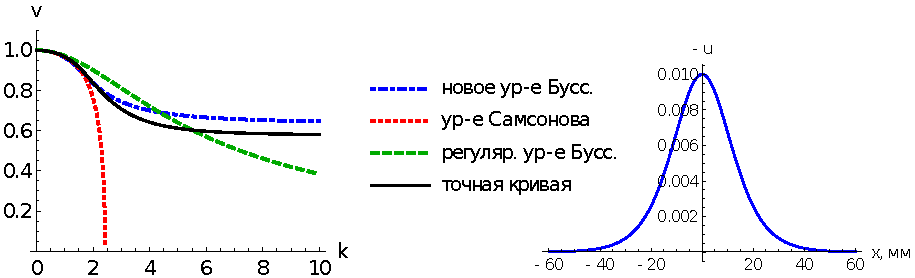
\includegraphics[width=1.02\linewidth]{Figures/Disp_Sol}
\end{figure}

\end{frame}


\begin{frame}{Численная схема}
\begin{minipage}{\textwidth}
\begin{itemize}
	\item Псевдоспектральный метод: поиск в конечномерном пространстве функции, совпадающей с решением в точках коллокации.
	\item Точки коллокации --- узлы интерполяционной квадратуры Гаусса (Радо, Лобатто).
	\item Дискретизация по времени с помощью метода Рунге-Кутты (RK45).
\end{itemize}
\end{minipage}
\end{frame}


\begin{frame}{Сравнение моделей: эволюция волны}
\footnotesize
\begin{minipage}{\textwidth}
	\begin{minipage}[b]{0.6\textwidth}
		\animategraphics[width=\linewidth]{12}{SolAnim001/p}{0}{100}
	\end{minipage}
	\hfill
	\begin{minipage}[b]{0.39\textwidth}
		%\centering
		\begin{tabular}{|c|c|c|}
			\hline 
			Уравн. & Ампл. & Скор.  \\ 
			\hline 
			Полные & 0.000966 & 1870.55 \\ 
			\hline 
			Буссин. & 0.000972 & 1870.58 \\ 
			\hline
			Отличие & 0.5\% & 0.0014\% \\
			\hline
		\end{tabular}
	 {\color{white}\vspace{2mm}123}
	\end{minipage}
\end{minipage}

\vspace{2mm}
\begin{minipage}{\textwidth}
	\begin{minipage}[b]{0.6\textwidth}
		\animategraphics[width=\linewidth]{12}{SolAnim010/p}{0}{90}
	\end{minipage}
	\hfill
	\begin{minipage}[b]{0.39\textwidth}
		\centering
		\begin{tabular}{|c|c|c|}
			\hline 
			Уравн. & Ампл. & Скор.  \\ 
			\hline 
			Полные & 0.0121 & 1894 \\ 
			\hline 
			Буссин. & 0.0128 & 1895 \\ 
			\hline 
			Отличие & 5.7\% & 0.2\% \\
			\hline
		\end{tabular}
		{\color{white}\vspace{2mm}123}
	\end{minipage}
\end{minipage}

\vspace{2mm}
\begin{minipage}{\textwidth}
	\begin{minipage}[b]{0.6\textwidth}
		\animategraphics[width=\linewidth]{12}{SolAnim050/p}{0}{150}
	\end{minipage}
	\hfill
	\begin{minipage}[b]{0.39\textwidth}
		\centering
		\begin{tabular}{|c|c|c|}
			\hline 
			Уравн. & Ампл. & Скор. \\ 
			\hline 
			Полные & 0.065 & 1968 \\ 
			\hline 
			Буссин. & 0.082 & 2049 \\ 
			\hline 
			Отличие & 26\% & 4.1\% \\
			\hline
		\end{tabular}
		{\color{white}\vspace{2mm}123}
	\end{minipage}
\end{minipage}
\end{frame}


\begin{frame}{Сравнение моделей: скорость-амплитуда}
\begin{wrapfigure}[10]{r}{200pt}
	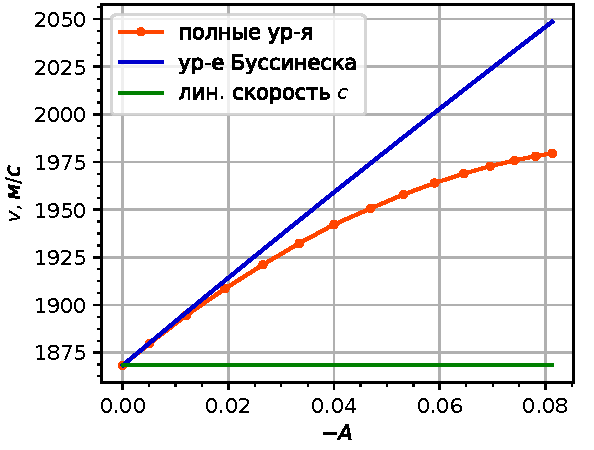
\includegraphics[width=\linewidth]{Figures/VelAmplColor}
\end{wrapfigure}
Зависимость скорости от амплитуды в модели Буссинеска:
\begin{equation}\nonumber
v(A) = c\sqrt{1 + A\frac{2\beta_1}{3}}
\end{equation}
Зависимость для полных уравнений получена в серии численных экспериментов.\\
\end{frame}


\begin{frame}{Сравнение моделей: удар по поверхности}
\begin{minipage}{\textwidth}
	\begin{minipage}[b]{0.65\textwidth}
		\flushleft
		Удар по боковой поверхности:
		\animategraphics[width=\linewidth]{100}{NormSurfImpact/p}{0}{90}
	\end{minipage}
	\hfill
	\begin{minipage}[b]{0.34\textwidth}
		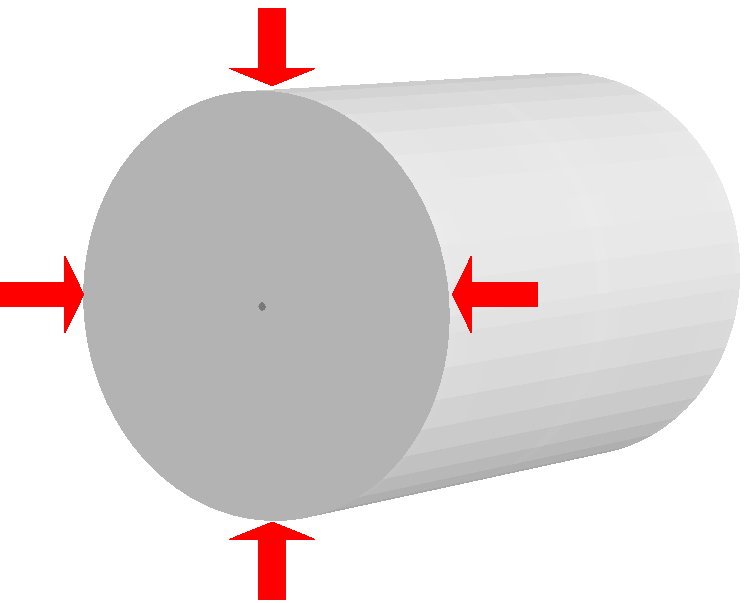
\includegraphics[width=\linewidth]{Figures/ImpactScheme2}
	\end{minipage}
\end{minipage}

\vspace{2mm}
\begin{minipage}{\textwidth}
	\begin{minipage}[b]{0.65\textwidth}
		\flushleft
		Удар по торцу:
		\animategraphics[width=\linewidth]{100}{FaceImpact/p}{0}{139}
	\end{minipage}
	\hfill
	\begin{minipage}[b]{0.34\textwidth}
		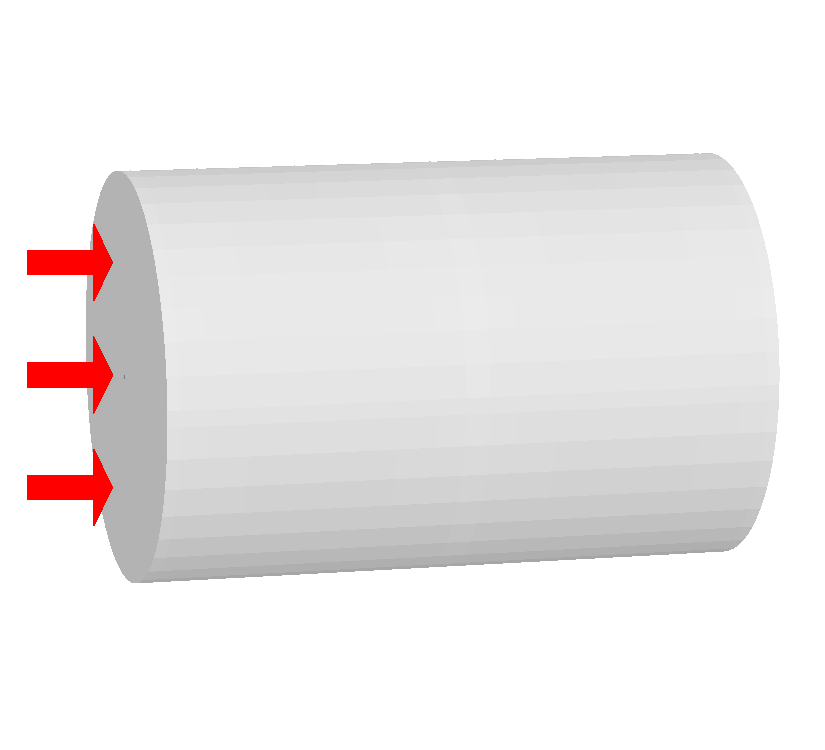
\includegraphics[width=\linewidth]{Figures/ImpactScheme}
	\end{minipage}
\end{minipage}
\end{frame}


\begin{frame}{Заключение}
\begin{itemize}
	\item Выведено 
	новое асимптотическое уравнение типа Буссинеска с~внешним воздействием, описывающая продольные волны в~нелинейно упругих стержнях круглого сечения.
	\item Построен метод, позволяющий численно моделировать полные уравнения движения стержня в рамках нелинейной теории упругости.
	\item Численно решён ряд начально-краевых задач, показывающих применимость выведенного уравнения типа Буссинеска для моделирования возникновения солитонов деформации.
\end{itemize}
\end{frame}


\begin{frame}{Статьи и конференции}
\small
Результаты работы частично опубликованы:
\footnotesize
\begin{itemize}
	\item Garbuzov F.\,E., Khusnutdinova K.\,R., Semenova I.\,V., On Boussinesq-type models for long longitudinal waves in elastic rods, \textit{Wave Motion} 88 (2019) 129--143.
\end{itemize}
\small
Публикации по смежным темам:
\footnotesize
\begin{itemize}
	\item Samsonov A.\,M., Semenova I.\,V., Garbuzov F.\,E.,  Nonlinear guided bulk waves in heterogeneous elastic structural elements. \textit{Int. J. Nonlin. Mech.} 94 (2017) 343--350.
	\item Semenova I.\,V., Belashov A.\,V., Garbuzov F.\,E., Samsonov A.\,M., Semenov A.\,A., Bulk strain solitons as a tool for determination of the third order elastic moduli of composite materials. \textit{Proceedings of SPIE 10329} (2017) 103291W.
	\item Гарбузов Ф.\,Е., Самсонов А.\,М., Семёнов А.\,А., Шварц А.\,Г., Определение упругих модулей	3-го порядка по параметрам объёмных солитонов деформации, \textit{ПЖТФ} 42\,(2) (2016) 121--123.
\end{itemize}
\small
Конференции:
\footnotesize
\begin{itemize}
	\item Days on Diffraction, C.-Петербург, 4 -- 8 июня 2018.
	\item Научная школа ''Нелинейные волны 2018'', Н. Новгород, 26 февр. -- 4 марта 2018.
	\item Nonlinear Waves Workshop, C.-Петербург, 22 декабря 2017.
\end{itemize}
\end{frame}



\appendix

\begin{frame}{Уравнения движения в безразмерной форме}
\small
\begin{equation} \nonumber
\begin{split}
&\rho c^2 U_{0tt} - (\lambda + 2\mu) U_{0xx} - 2(\lambda + \mu) V_{1x} - 4\mu U_2 + \Phi_1(U_0, V_1, U_2) \varepsilon\\
&\quad+ \left[\rho c^2 U_{2tt} - (\lambda + 2\mu)U_{2xx} - 4(\lambda + \mu)V_{3x} - 16\mu U_4\right] r^2 + O(\varepsilon^2, \varepsilon r^2, r^4) = 0,
\end{split}
\end{equation}
\begin{equation} \nonumber
\begin{split}
&r \big( \rho c^2 V_{1tt} - \mu V_{1xx} - 2(\lambda + \mu)U_{2x} - 8(\lambda + 2\mu)V_3 - \Phi_2(U_0, V_1, U_2, V_3)\varepsilon \\
&\quad- \left[\rho c^2 V_{3tt} - \mu V_{3xx} - 4(\lambda + \mu)U_{4x} - 24(\lambda + 2\mu)V_5 \right] r^2  + O(\varepsilon^2, \varepsilon r^2, r^4)\big) = 0,
\end{split}
\end{equation}
\normalsize
$\Phi_1$, $\Phi_2$ --- нелинейные функции своих аргументов.\\
Неизвестные функции ищутся в виде $U_2 = U_2^{(0)} + \varepsilon U_2^{(1)} + \dots$
\small
\begin{align*}
U_2 &= \frac{1}{4\mu} \left[ \rho c^2 U_{0tt} - (\lambda + 2\mu) U_{0xx} - 2(\lambda + \mu) V_{1x} \right] + \varepsilon U_2^{(1)}(x,t) + O(\varepsilon^2),\\
V_3 &= \frac{1}{8(\lambda + 2\mu)} \left[ \rho c^2 V_{1tt} - 2(\lambda + \mu) U_{2x} - \mu V_{1xx} \right] + \varepsilon V_3^{(1)}(x,t) + O(\varepsilon^2),\\
U_4 &= \frac{1}{16\mu}\left[\rho c^2 U_{2tt} - (\lambda + 2\mu) U_{2xx} - 4(\lambda + \mu) V_{3x}\right] + O(\varepsilon),\\
V_5 &= \frac{1}{24(\lambda + 2\mu)} \left(\rho c^2 V_{3tt} - 4(\lambda+\mu)U_{4x} - \mu V_{3xx}\right) + O(\varepsilon).
\end{align*}
\end{frame}

\begin{frame}{Граничные условия}
На границе задано нормальное напряжение $P(x,t)$ и касательное $T(x,t)$:
\small
\begin{align*} \nonumber
\begin{split}
&2 (\lambda + \mu) {\color{black}V_1} + \lambda {\color{black}U_{0x}} +\varepsilon \lb b_1 {\color{black}U_{0x}^2} + b_2 {\color{black}U_{0x}}{\color{black}V_1} + b_3 {\color{black}V_1^2} \rb + \delta^2 \bigg[ a_1 {\color{black}U_{0xxx}} + a_2 {\color{black}U_{0xtt}} +\\
&\hspace{40mm}+ a_3 {\color{black}V_{1tt}} + a_4 {\color{black}V_{1xx}}\bigg] + O(\varepsilon^2, \varepsilon\delta^2, \delta^4) =  \frac{\mu(3\lambda + 2\mu)}{\lambda + \mu} P,
\end{split}\\
\begin{split}
&\rho  c^2 {\color{black}U_{0tt}} -2 \lambda {\color{black}V_{1x}}-(\lambda +2 \mu ) {\color{black}U_{0xx}} - \varepsilon \lb b_4 {\color{black}U_{0x}^2} + b_5 {\color{black}U_{0x}}{\color{black}V_1} + b_6 {\color{black}V_1^2} \rb_x + \delta^2\bigg[a_5 {\color{black}U_{0xxxx}} +\\
&\hspace{2mm}+ a_6 {\color{black}U_{0tttt}} + a_7 {\color{black}U_{0xxtt}} + a_8 {\color{black}V_{1xxx}} + a_9 {\color{black}V_{1xtt}} \bigg] + O(\varepsilon^2, \varepsilon\delta^2, \delta^4) = \frac{2\mu(3\lambda + 2\mu)}{\lambda + \mu} T.
\end{split}
\end{align*}
Коэффициенты $a_j$, $b_j$ зависят от упругих модулей.\\
\vspace{1mm}
\normalsize
Исключение ${\color{black}V_1}$ приводит к одномерному уравнению типа Буссинеска.
\end{frame}


\begin{frame}{Многодоменный псевдоспектральный метод}
	\hspace*{-2mm}
	\begin{minipage}{1.02\textwidth}
		\begin{itemize}
			\item Спектральное представление: $\vect{U}(x,r,t) = \displaystyle\sum_{n,m} \vect{\widehat{U}}_{nm}(t) \Phi_{n}(x) \Psi_{m}(r)$.
			\item Пространственные производные вычисляются умножением массива значений функций на матрицу дифференцирования --- медленно при большом количестве точек.
			\item Для ускорения: многодоменный псевдоспектральный метод.
		\end{itemize}
	\end{minipage}

	\begin{figure}
		\centering
		\begin{subfigure}{0.5\textwidth}
			\flushleft
			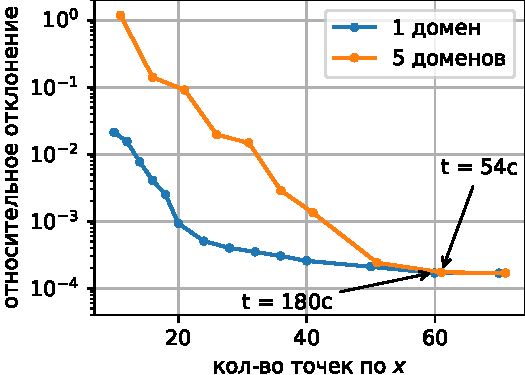
\includegraphics[width=.95\textwidth]{Figures/Error}
		\end{subfigure}
		\begin{subfigure}{0.45\textwidth}
			\centering
			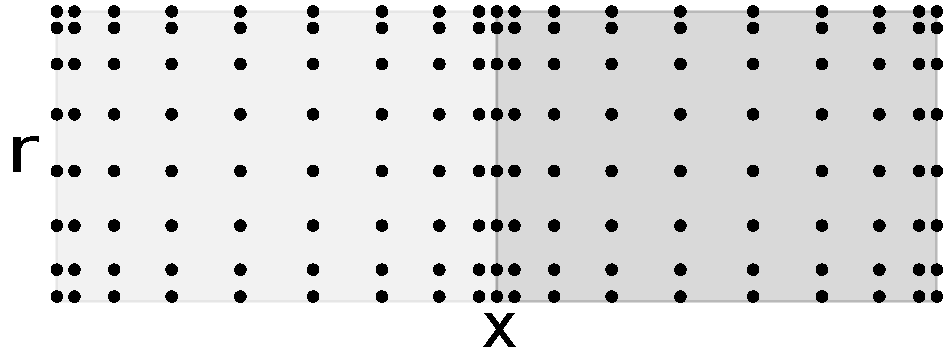
\includegraphics[width=\textwidth]{Figures/Grid2D}\\
			\footnotesize
			Пример двумерной сетки
		\end{subfigure}
	\end{figure}
\end{frame}

\begin{frame}{Эксперимент}
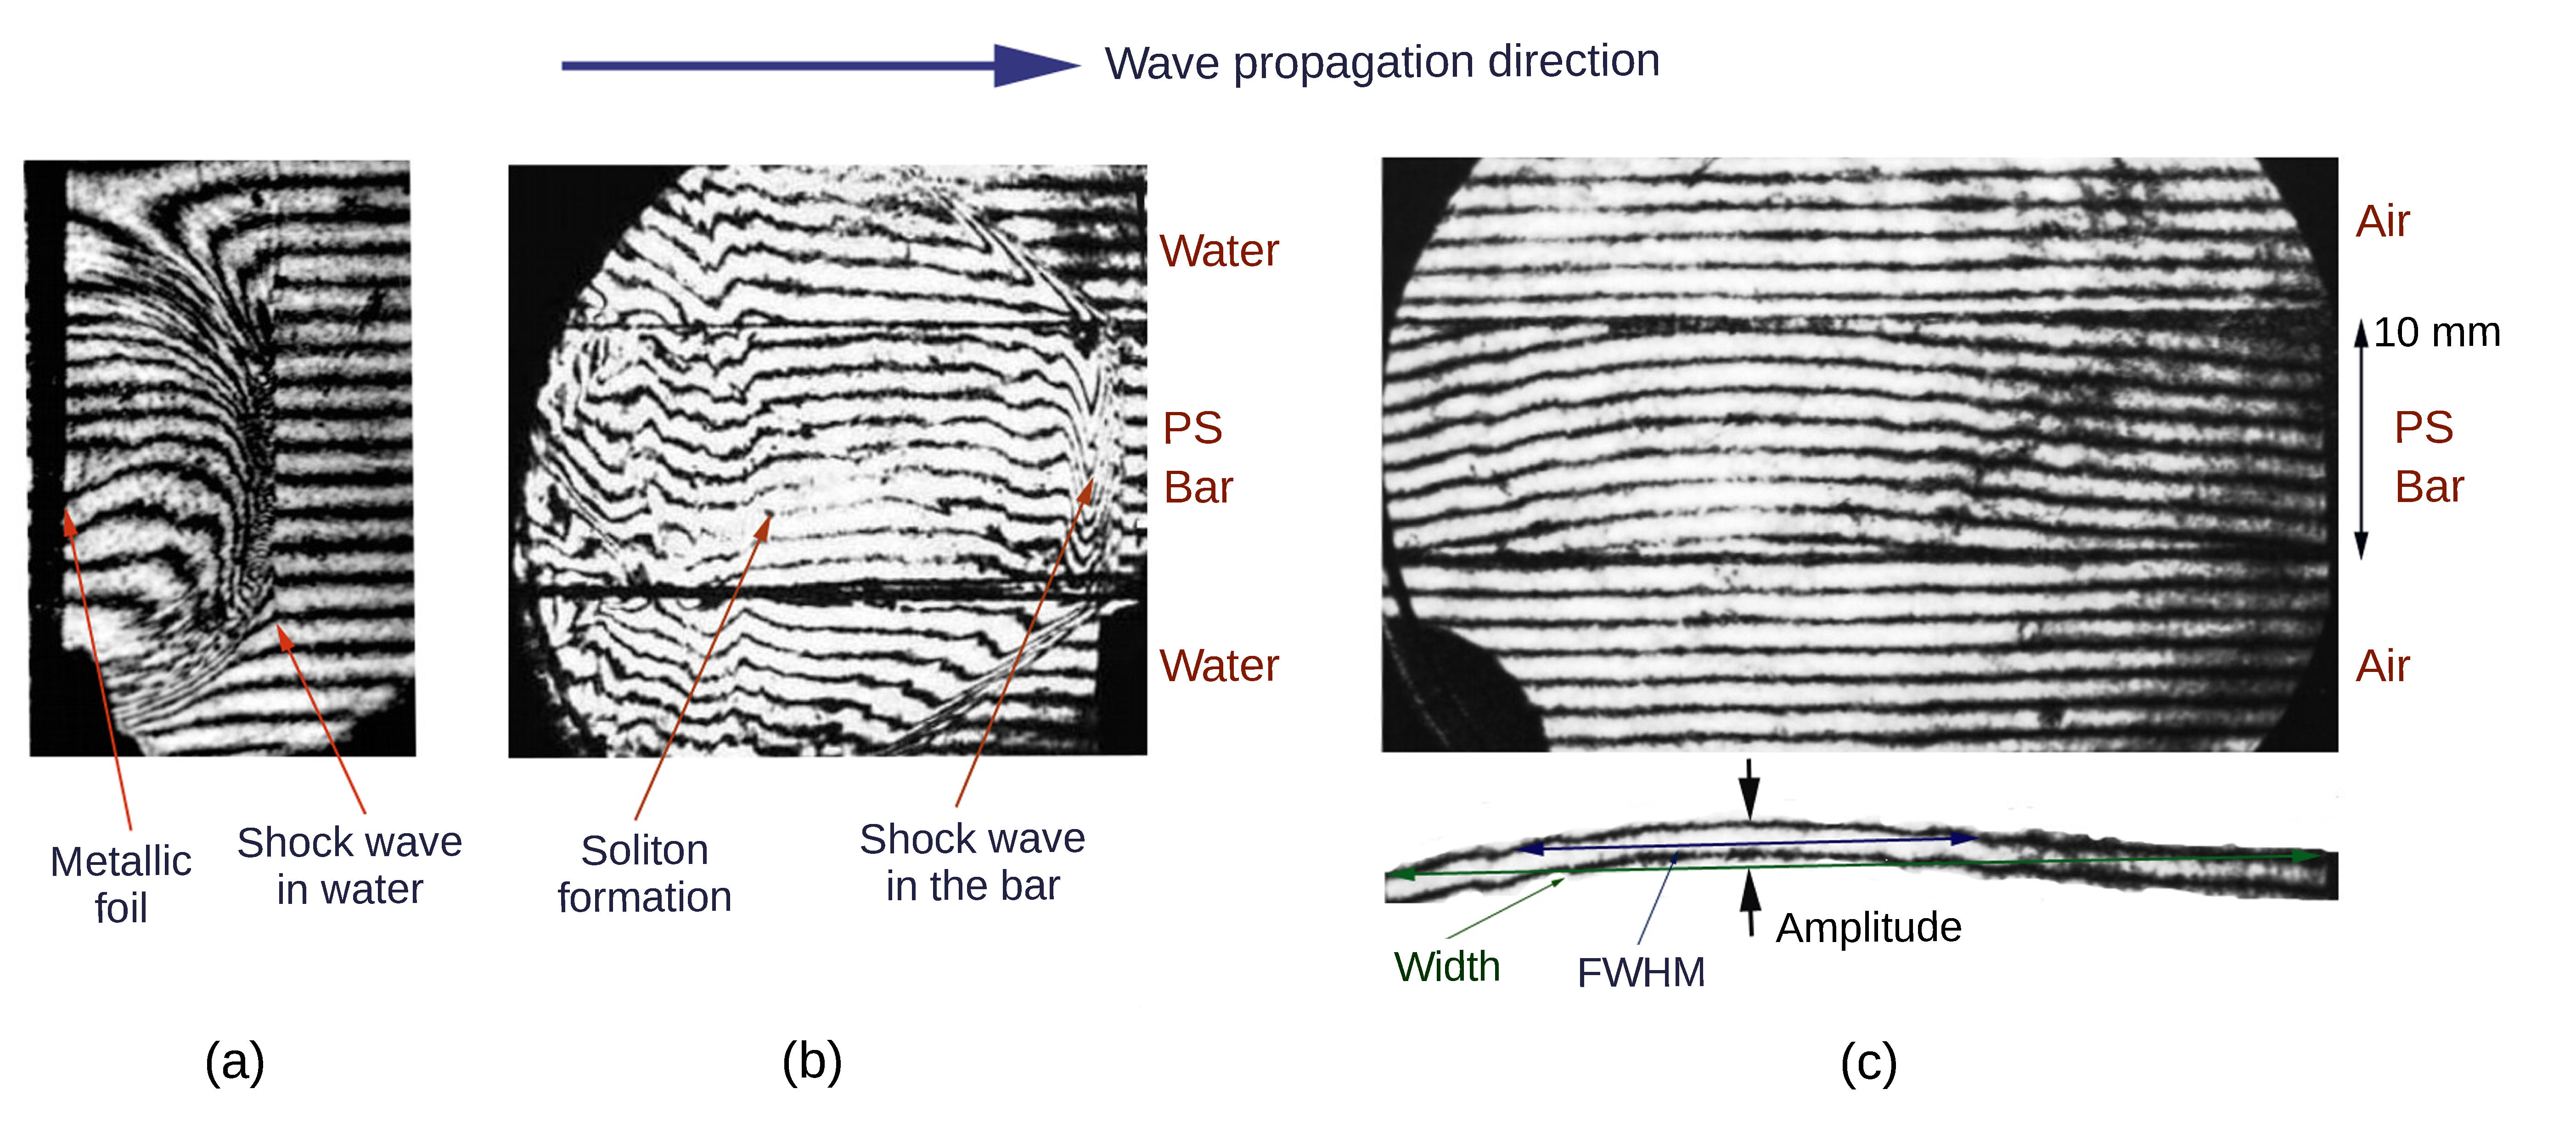
\includegraphics[width=1.05\linewidth]{Figures/trio_2_300_2}
\end{frame}


\begin{frame}{Трёхмерная сетка}
\begin{figure}[h!]
		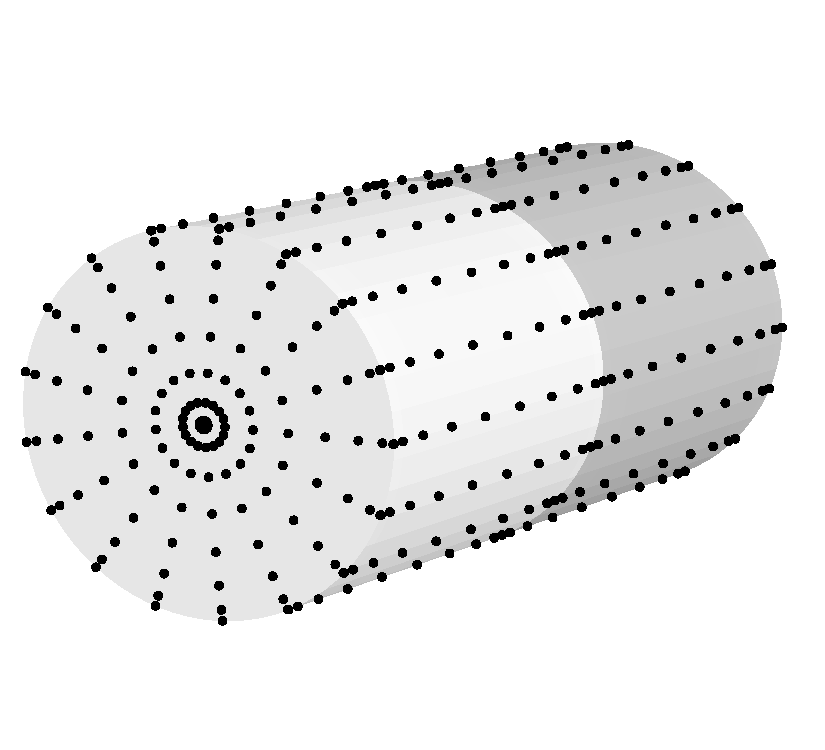
\includegraphics[width=.5\linewidth]{Figures/Grid3D}
\end{figure}
\end{frame}

\end{document}